\chapter{Supporting Materials}

\begin{figure}
\centering
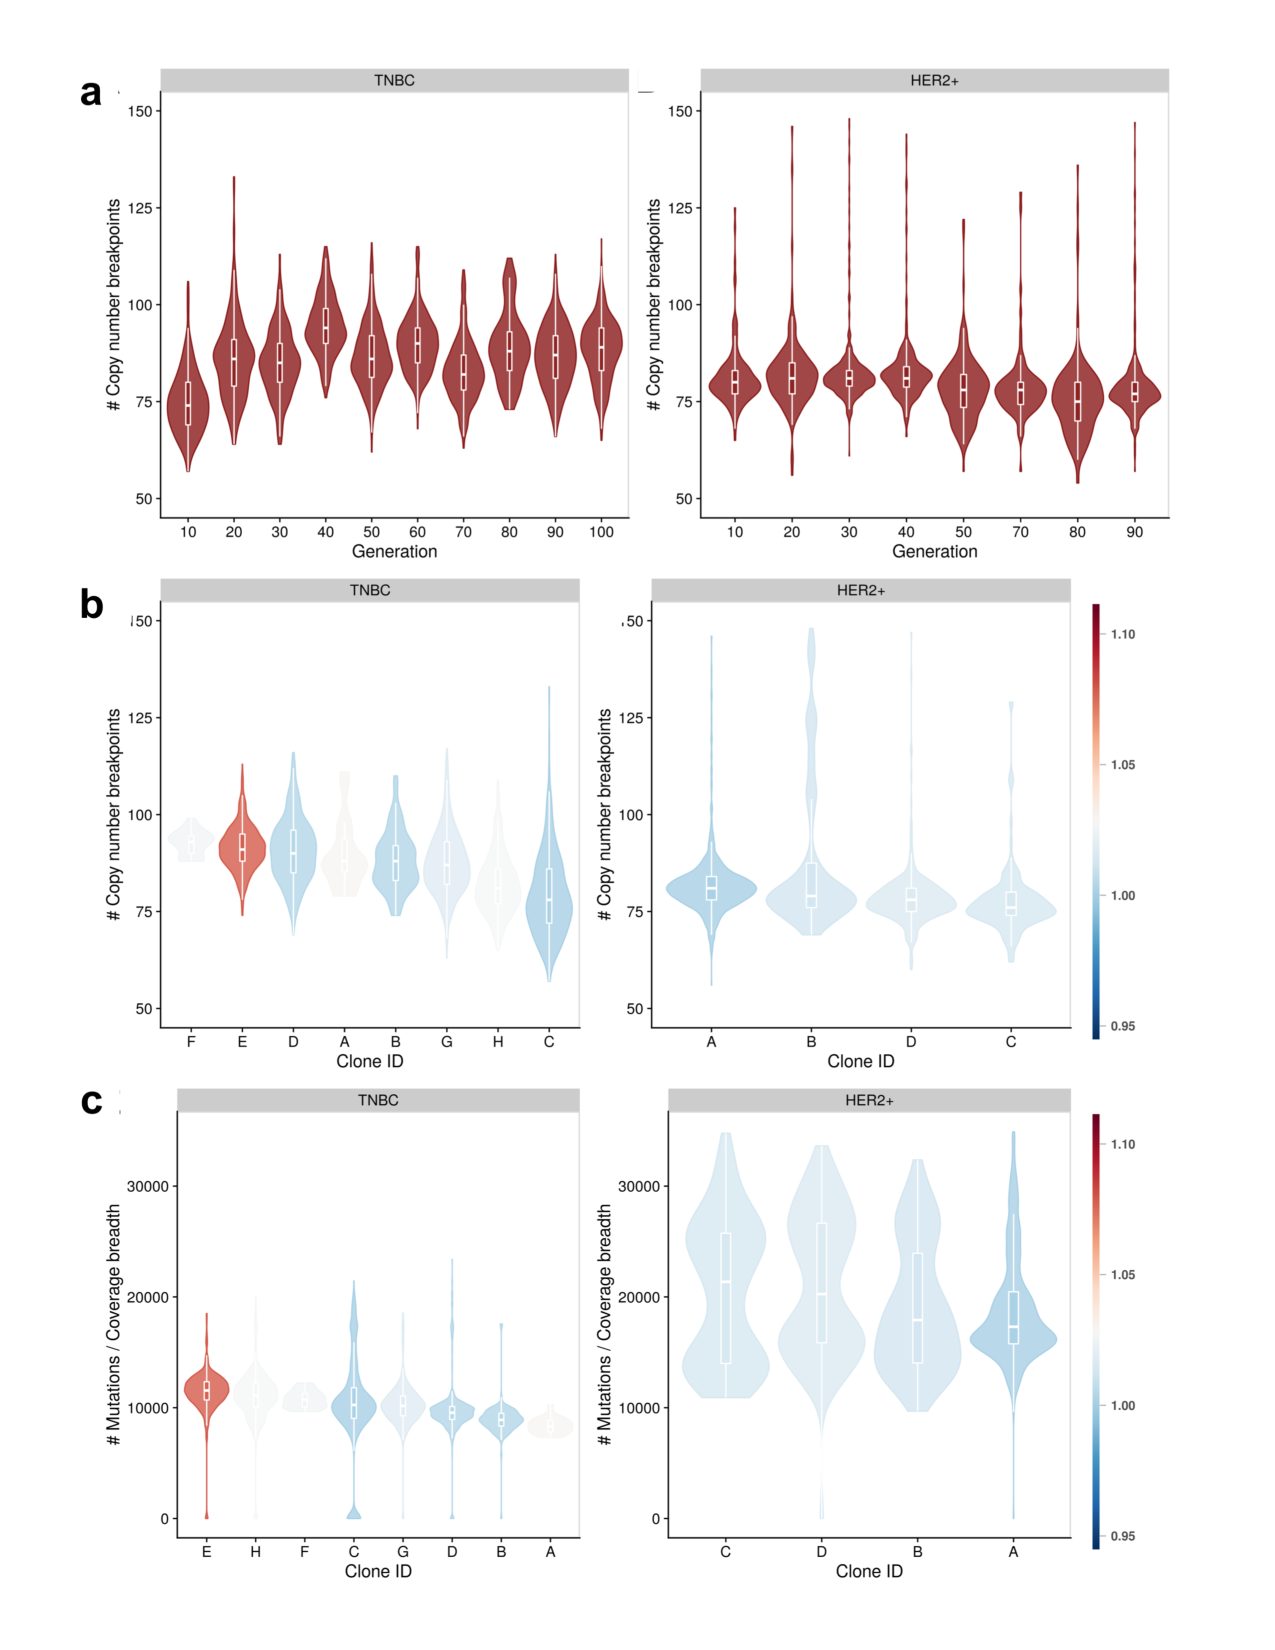
\includegraphics[width=\textwidth]{Figures/mutationanalysisbreakpoints.pdf}
  \caption[Structural variant and mutation rates of HER2+ and TNBC PDX]
	{\small
	\textbf{Structural variant and mutation rates of HER2+ and TNBC PDX.}
	    \textbf{(a)} Distribution over copy number
breakpoints/cell as a function of generation for left: TNBC, right: HER2+
   \textbf{(b)} Clone specific distributions over copy number breakpoints/cell, coloured by fitness coefficients for left: TNBC, right: HER2+
    \textbf{(c)} Clone specific distributions over point mutations/cell, coloured by fitness coefficients for left:TNBC, right:HER2+
}
    \label{fig:mutationanalysisbreakpoints}
    \end{figure}



\begin{figure}
\centering
  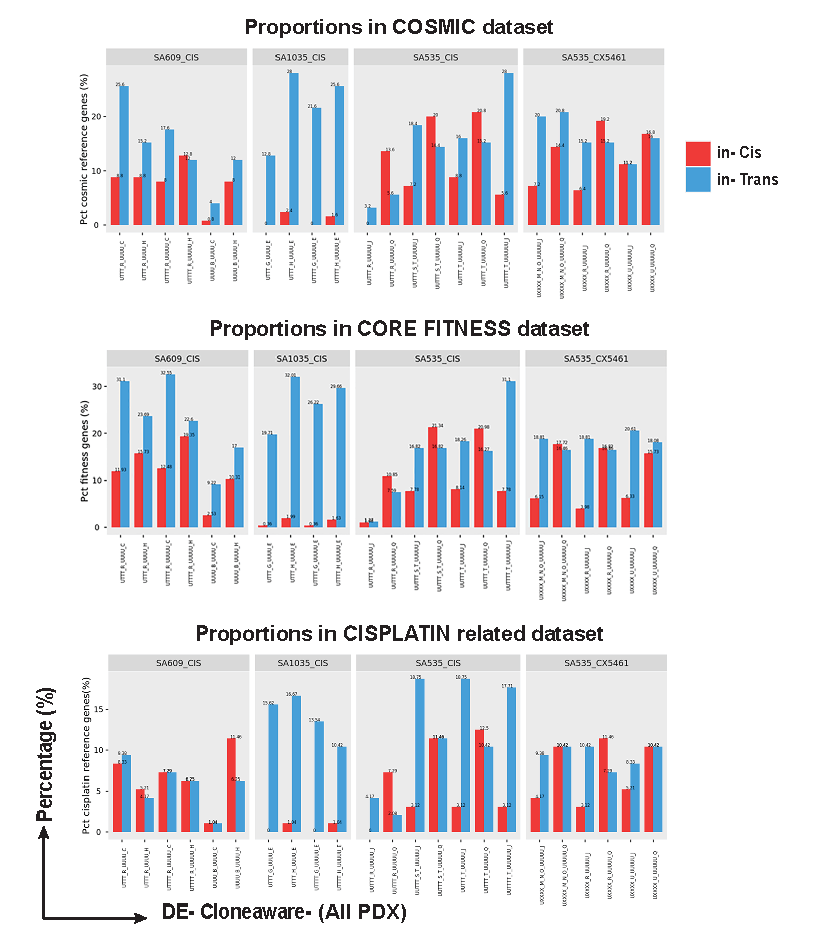
\includegraphics[width=\textwidth]{Figures/fig3_In_cispercentage.pdf}
	
\caption[Proportion of \textit{in cis} and \textit{in trans} regulated gene expression in scRNAseq data]
	{\small
	\textbf{Proportion of \textit{cis} and \textit{trans} regulated gene expression in scRNAseq data.}
	   Horizontal axis shows differential expression between two selected clones from all the three PDX treated and un-treated timeseries. Vertical axis gives percentage presence of genes \textit{in cis} or in trans. red bars represent in cis and blue bars represent in -trans regulated gene expression.
	   \textbf{(Upper)} This graph gives us percentage of genes by looking into the gene data set from COSMIC cancer gene dataset \cite{vogelstein2013cancer} that corresponds to our clone aware \ac{DE}.
	    \textbf{(Middle)} same like upper plot but looking into CORE FITNESS data set \cite{behan2019prioritization}.
	     \textbf{(Lower)} Same like above but looking into cisplatin related gene list curated from literature.
	    
	}
	\label{fig:fig3_In_cispercentage}
\end{figure}















\begin{figure}
\centering
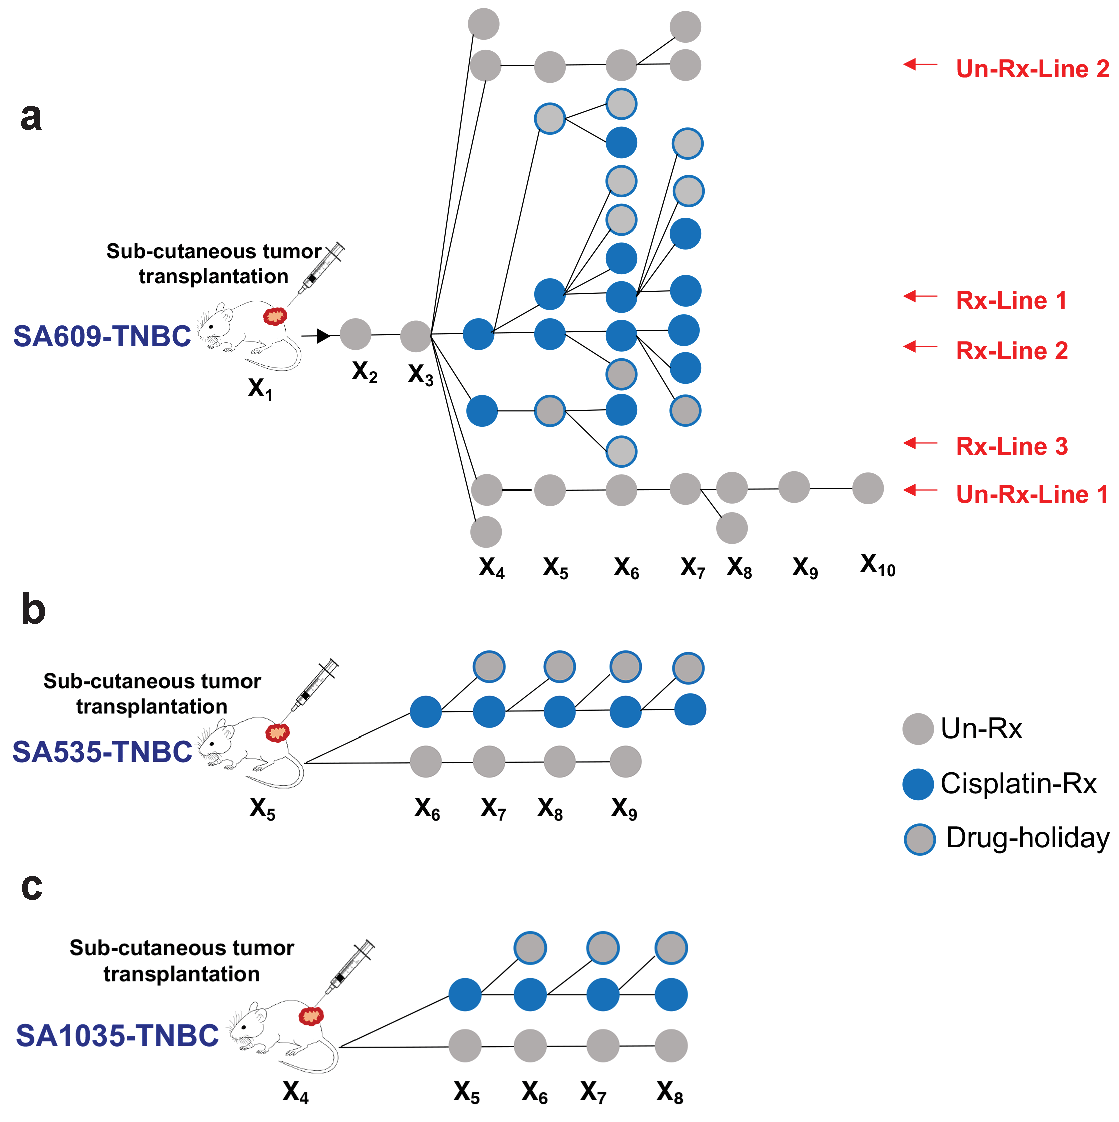
\includegraphics[width=\textwidth]{Figures/treatedtimeseriesmanuscript.pdf}
  \caption[TNBC PDX timeseries clonal dynamics under drug perturbations]
	{\small
	\textbf{TNBC PDX timeseries showing timepoint nodes used for single cell whole genome sequencing}
	     All nodes representing each PDX tumour were digested to acquire genomes of single cells (~200-600 cells/tumor). Extra replicate tumors at each time point are not shown in the diagram (n=2-4). Grey circles represent un-treated, blue represents Cisplatin treated and grey with blue outline presents drug-holiday samples 
	     \textbf{(a)} SA609-TNBC time series with replicates. DLP+ collected starting from X1 to X10 (Un-Rx line 1). Top grey branch indicating Un-Rx line 2. The middle three branches are cisplatin treated time series replicate branches 
	     \textbf{(b)} SA535-TNBC  showing the tumor nodes taken for DLP+ starting from X5 untreated  \textbf{(c)} SA1035-TNBC  showing the tumor nodes taken for DLP+ starting from X 4 untreated.}
     \label{fig:treatedtimeseriesmanuscript}

\end{figure}




\begin{figure}
\centering
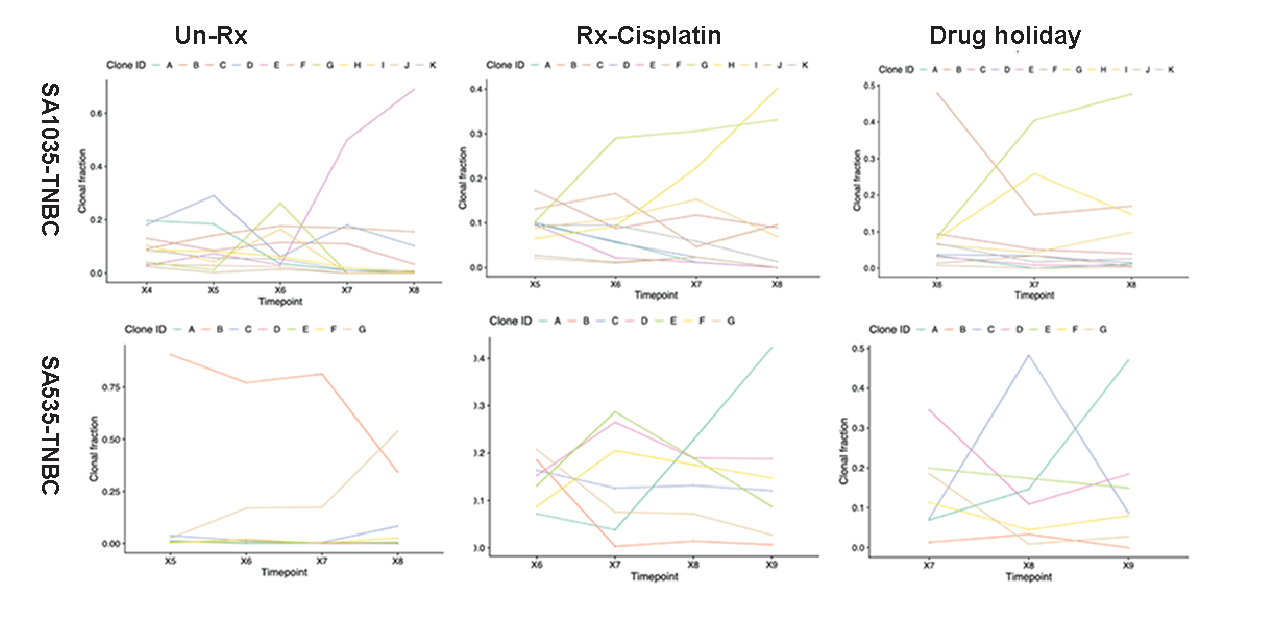
\includegraphics[width=\textwidth]{Figures/drugholidaysamples.pdf}
	
\caption[TNBC-SA609 PDX reproducible clonal dynamics with and without treatment]
	{\small
\textbf{Observed trajectories including drug-holiday samples.}
Panels showing line trajectories of clonal behaviour over time in two additional TNBC all three conditions. Fitness reversal in drug holiday samples of SA1035 and SA535 were not very prominent as compare to SA609. Horizontal axis representing the timepoints of each generation and vertical axis shows clonal fractions.
	}
	\label{fig:drugholidaysamples}
\end{figure}



\begin{figure}
\centering
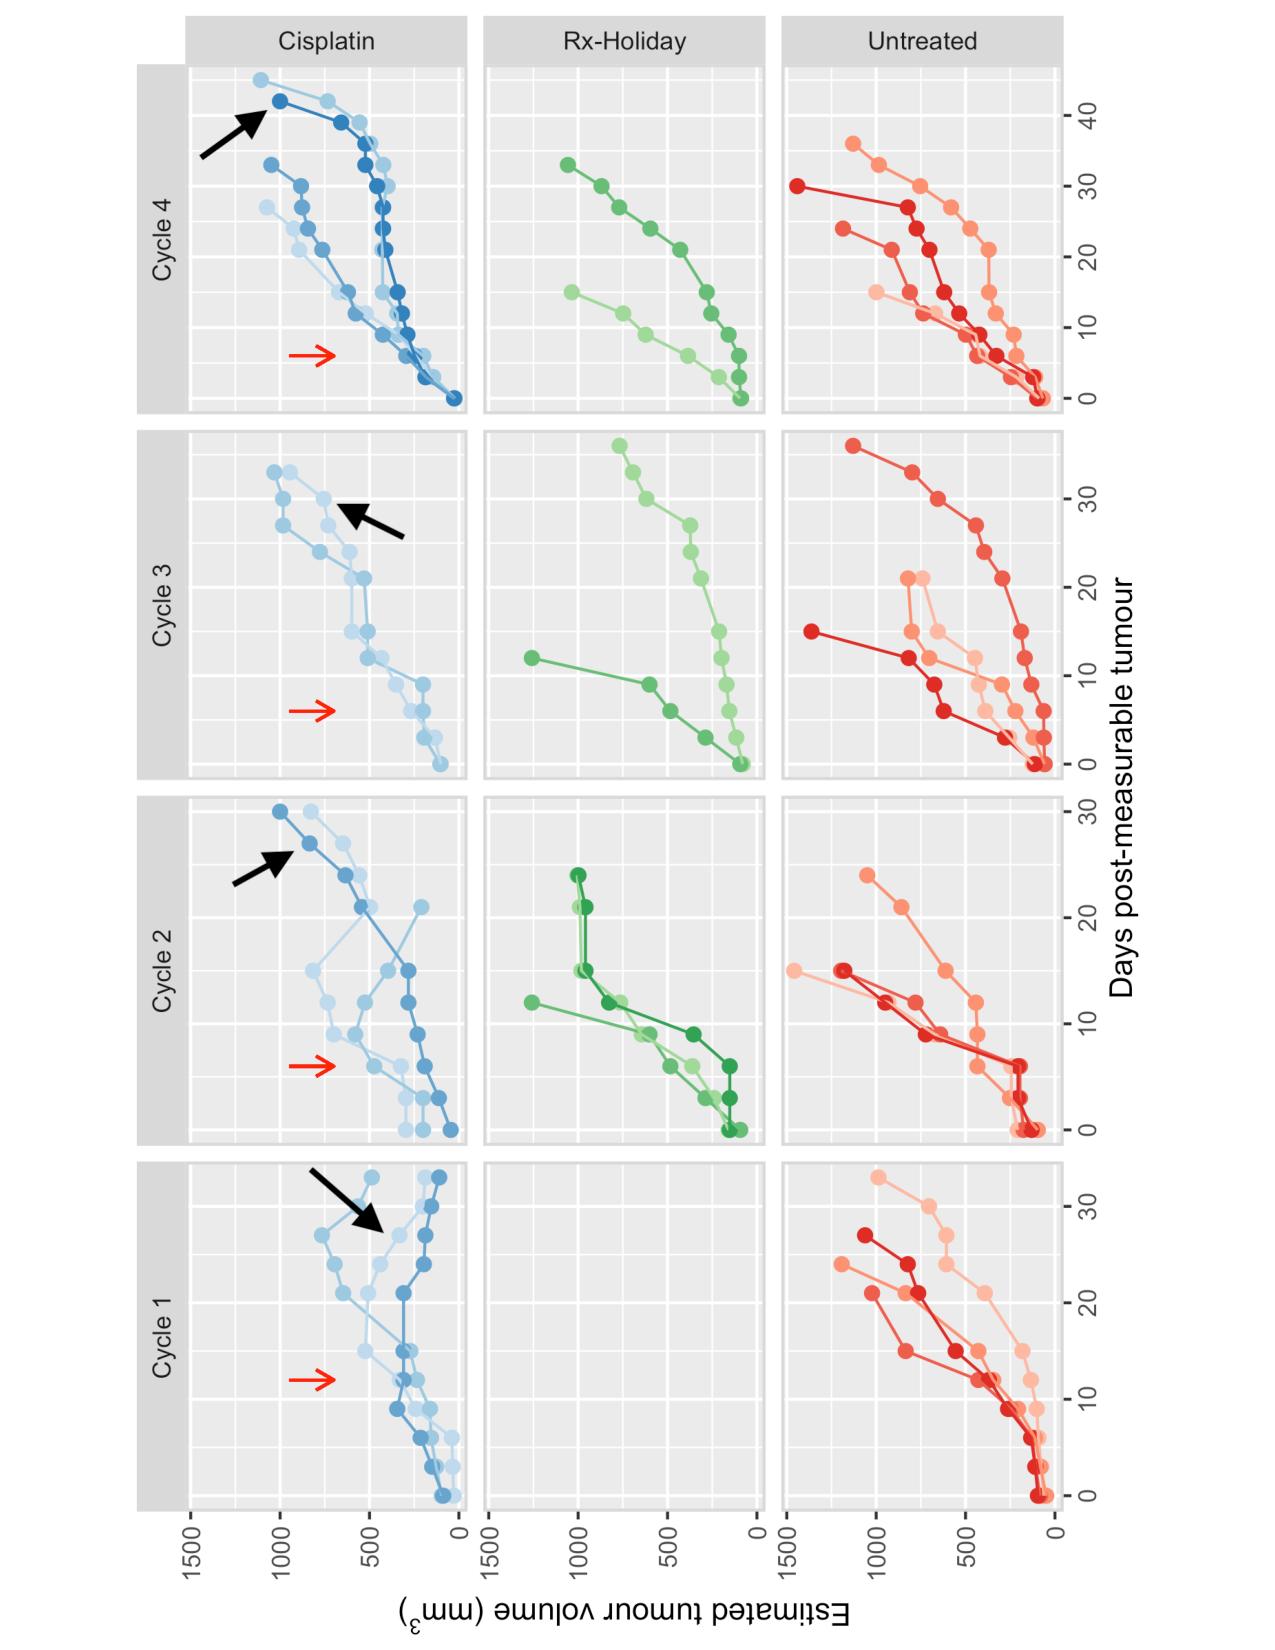
\includegraphics[width=\textwidth]{Figures/SA1035_AllCyclesCisplatin.pdf}
	
\caption[Tumor growth curves from SA1035 TNBC PDX]
	{\small
\textbf{Tumor growth curves from SA1035 TNBC PDX.}
Tumour response curves in each cycle of cisplatin treatment in SA1035 TNBC PDX. The vertical axis on right indicates tumor status and on left shows tumor volume. Horizontal axis presents days post measurable tumor.
}
	\label{fig:SA1035_AllCyclesCisplatin}
\end{figure}


 % Table generated by Excel2LaTeX from sheet 'Sheet1'
 \begin{table}[htbp]
   \centering
   \caption{Cisplatin related genes from last 10 years literature}
     \begin{tabular}{|l|l|l|l|r}
     
     \hline
     \multicolumn{4}{|l|}{Gene Names}  \\
     \hline
     
     VCAM1  & GCS    & BRCA2  & XAF1    \\
     VIM    & GST    & VDAC   & DYRK1B  \\
     SLC31A1 & MT     & BAX    & ERBB2 \\
     GST    & ERCC1  & BCL    & HSPs   \\
     HMGB   & MLH1   & BIRC5  & TMEM205 \\
     CTR1   & MSH2   & CPN    & PDGFR \\
     ATP7A  & POLH   & CASP   & IGF1R  \\
     ATP7B  & REV3   & MAPKs  & TRP14  \\
     MRP2   & REV7   & p63    & RAB7   \\
     GSH    & BRCA1  & TP53   & RAB8   \\
     \hline
     \end{tabular}%
   \label{tab:Cisplatinrelatedgenes}%
 \end{table}
 
 
 
\begin{figure}
\centering
  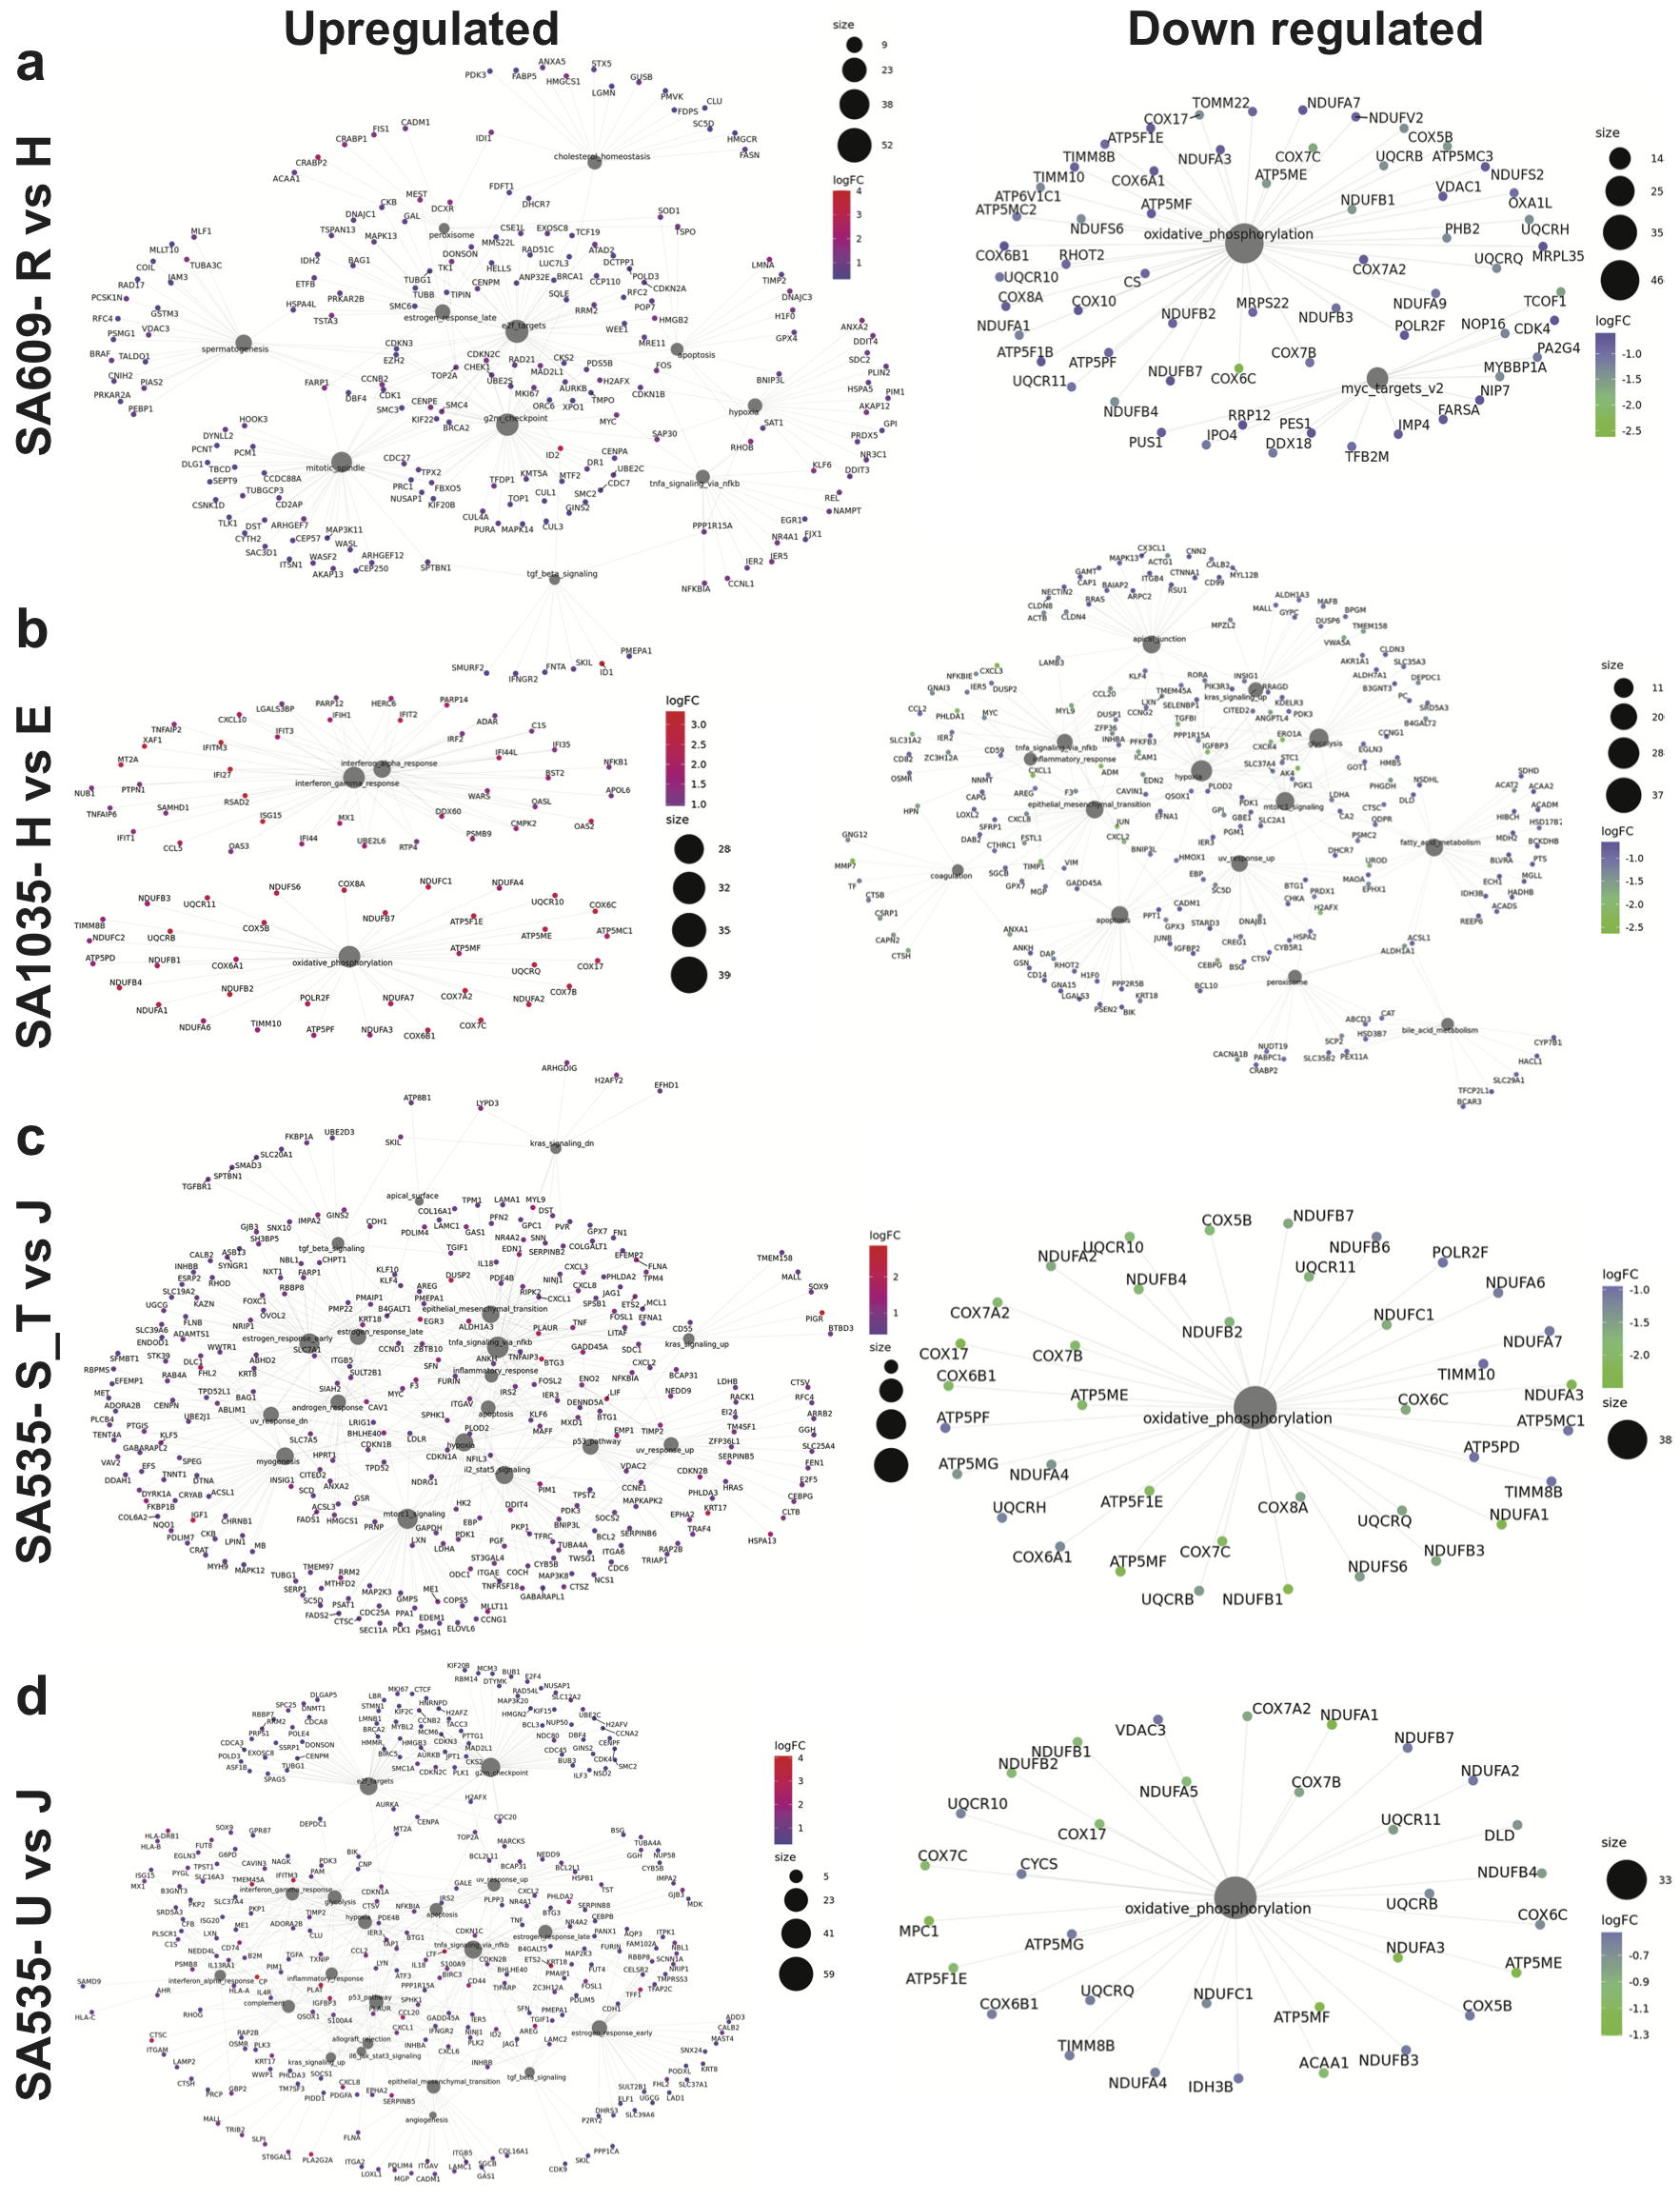
\includegraphics[width=\textwidth]{Figures/genenetworkanalysis.pdf}
\caption[DE of resistant and sensitive clonealign defined clones]
	{\small
	\textbf{Gene network analysis denoting connections of up-and-down regulated pathways across timeseries PDX}. Size of black circle indicates the number of genes, colour bars indicate the log fold change.
	\textbf{(a-d)} Genes in resistant vs sensitive clones of SA609, SA1035, SA535 (cisplatin and CX-5461 treated), respectively}
	   	\label{fig:genenetworkanalysis}
\end{figure} 
 
 
 
 
 
 

\begin{figure}
\centering
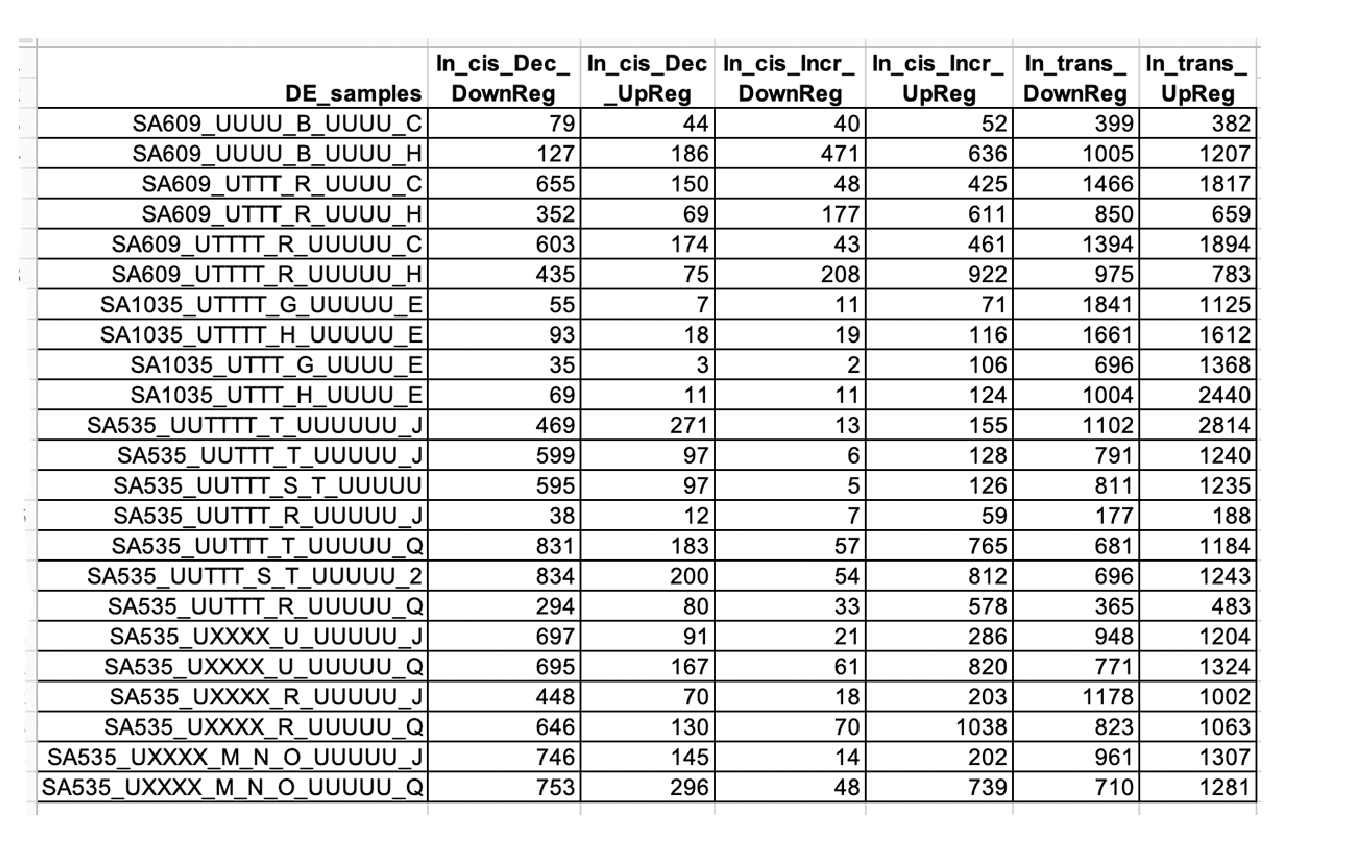
\includegraphics[width=\textwidth]{Figures/Appendixtable.pdf}
\caption[Summary of number of genes \textit{in-cis} and \textit{in-trans}]
	{\small
	\textbf{Summary of number of genes \textit{in-cis} and \textit{in-trans}.}
	  Summary of number of genes up and down regulated within our data set with respect to the reference genes.

}
    \label{fig:Appendixtable}
    \end{figure}
    
   
   
 
 
 % Please add the following required packages to your document preamble:
% \usepackage{graphicx}
% \usepackage{lscape}
\begin{landscape}
\begin{table}[]
\caption{All PDX-TMA scoring of IHC staining}
\label{tab:my-table}
\resizebox{1.5\textwidth}{!}{%
\begin{tabular}{lllllllllllllllllllllllllllllllllllllllll}
Timeseries/TMA1 &
  Timepoints &
  Treatment status &
  ER intensity &
  ER \% &
  PR intensity &
  PR \% &
  HER 2 intensity &
  HER 2 \% &
  Ki67 intensity &
  Ki67 \% &
  EGFR intensity &
  EGFR \% &
  SMA intensity &
  SMA \% &
  CK8 intensity &
  CK8 \% &
  CK14 intensity &
  CK14 \% &
  CK5/6 intensity &
  CK5/6 \% &
  E-cad intensity &
  E-cad \% &
  comments &
   &
  vimentin intensity &
  vimentin \% &
  slug/snail intensity &
  slug/snail \% &
  twist intensity &
  twist \% &
  INPP4B intensity &
  INPP4B \% &
  Masson trichrome &
  comments &
   &
   &
   &
   &
   &
   \\
HER2+ &
  X1 &
  Un-Rx &
  0 &
  0 &
  0 &
  0 &
  1+ &
  30 &
  3+ &
  60 &
  0 &
  0 &
  3+ &
  0-1 &
  1+ &
  10 &
  3+ &
  80 &
  3+ &
  70 &
  0 &
  0 &
  HER2? &
   &
  0 &
  0 &
  1+ &
  70 &
  0 &
  0 &
  0 &
  0 &
  2+ &
  most tumor disappered in INPP4B restain &
   &
   &
   &
   &
   &
   \\
HER2+ &
  X2 &
  Un-Rx &
  0 &
  0 &
  0 &
  0 &
  1+ &
  30 &
  3+ &
  60 &
  0 &
  0 &
  3+ &
  5 &
  1+ &
  1-5 &
  3+ &
  60 &
  3+ &
  80 &
  0 &
  0 &
   &
   &
  3+ &
  0-1 &
  1+ &
  80 &
  0 &
  0 &
  1+ &
  1 &
  1+ &
   &
   &
   &
   &
   &
   &
   \\
HER2+ &
  X3 &
  Un-Rx &
  1+ &
  0-1 &
  0 &
  0 &
  2+ &
  30 &
  2+ &
  30 &
  0 &
  0 &
  3+ &
  1-5 &
  2+ &
  20 &
  3+ &
  20 &
  3+ &
  50 &
  0 &
  0 &
   &
   &
  3+ &
  0-1 &
  1+ &
  70 &
  0 &
  0 &
  1+ &
  0-1 &
  2+ &
   &
   &
   &
   &
   &
   &
   \\
HER2+ &
  X4 &
  Un-Rx &
  0 &
  0 &
  0 &
  0 &
  1+ &
  10 &
  3+ &
  70 &
  0 &
  0 &
  3+ &
  20 &
  1+ &
  1-5 &
  3+ &
  1-5 &
  3+ &
  20 &
  0 &
  0 &
   &
   &
  3+ &
  0-1 &
  2+ &
  70 &
  0 &
  0 &
  1+ &
  0-1 &
  1+ &
   &
   &
   &
   &
   &
   &
   \\
HER2+ &
  X5 &
  Un-Rx &
  0 &
  0 &
  0 &
  0 &
  0 &
  0 &
  3+ &
  70 &
  1+ &
  5 &
  3+ &
  1 &
  1+ &
  1-5 &
  2+ &
  1 &
  2+ &
  10 &
  3+ &
  60 &
  E-cad nega area artifact? &
   &
  3+ &
  0-1 &
  1+ &
  50 &
  0 &
  0 &
  1+ &
  0-1 &
  0 &
   &
   &
   &
   &
   &
   &
   \\
HER2+ &
  X6 &
  Un-Rx &
  0 &
  0 &
  0 &
  0 &
  1+ &
  10 &
  3+ &
  70 &
  1+ &
  5 &
  2+ &
  1-5 &
  1+ &
  1 &
  3+ &
  1 &
  2+ &
  10 &
  3+ &
  30 &
  E-cad nega area artifact? &
   &
  3+ &
  0-1 &
  1+ &
  60 &
  3+ &
  0-1 &
  1+ &
  0-1 &
  0 &
   &
   &
   &
   &
   &
   &
   \\
HER2+ &
  X7 &
  Un-Rx &
  0 &
  0 &
  0 &
  0 &
  1+ &
  5 &
  3+ &
  50 &
  2+ &
  5 &
  2+ &
  1 &
  1+ &
  0-1 &
  3+ &
  1-5 &
  2+ &
  10 &
  3+ &
  70 &
   &
   &
  3+ &
  0-1 &
  1+ &
  20 &
  0 &
  0 &
  0 &
  0 &
  1+ &
   &
   &
   &
   &
   &
   &
   \\
HER2+ &
  X8 &
  Un-Rx &
  0 &
  0 &
  0 &
  0 &
  0 &
  0 &
  2+ &
  30 &
  0 &
  0 &
  1+ &
  40 &
  1+ &
  1-5 &
  3+ &
  5 &
  1+ &
  10 &
  3+ &
  80 &
   &
   &
  2+ &
  1 &
  0 &
  0 &
  0 &
  0 &
  0 &
  0 &
  2+ &
   &
   &
   &
   &
   &
   &
   \\
HER2+ &
  X9 &
  Un-Rx &
  0 &
  0 &
  0 &
  0 &
  2+ &
  20 &
  3+ &
  50 &
  2+ &
  5 &
  2+ &
  0-1 &
  1+ &
  5 &
  3+ &
  1 &
  3+ &
  20 &
  3+ &
  100 &
   &
   &
  3+ &
  1 &
  2+ &
  80 &
  3+ &
  0-1 &
  1+ &
  0-1 &
  1+ &
   &
   &
   &
   &
   &
   &
   \\
HER2+ &
  X10 &
  Un-Rx &
  0 &
  0 &
  0 &
  0 &
  1+ &
  20 &
  3+ &
  70 &
  1+ &
  10 &
  3+ &
  30 &
  1+ &
  1 &
  3+ &
  1-5 &
  3+ &
  20 &
  3+ &
  100 &
   &
   &
  3+ &
  1 &
  2+ &
  80 &
  3+ &
  0-1 &
  1+ &
  0-1 &
  1+ &
   &
   &
   &
   &
   &
   &
   \\
 &
   &
   &
   &
   &
   &
   &
   &
   &
   &
   &
   &
   &
   &
   &
   &
   &
   &
   &
   &
   &
   &
   &
   &
   &
   &
   &
   &
   &
   &
   &
   &
   &
   &
   &
   &
   &
   &
   &
   &
   \\
TNBC-SA609 &
  X1 &
  Un-Rx &
  0 &
  0 &
  1+ &
  5 &
  0 &
  0 &
  3+ &
  80 &
  0 &
  0 &
  2+ &
  1 &
  0 &
  0 &
  1+ &
  0-1 &
  2+ &
  0-1 &
  0 &
  0 &
   &
   &
  3+ &
  20 &
  1+ &
  60 &
  2+ &
  0-1 &
  0 &
  0 &
  0 &
  INPP4B nuclear+ &
   &
   &
   &
   &
   &
   \\
TNBC-SA609 &
  X2 &
  Un-Rx &
  0 &
  0 &
  1+ &
  0-1 &
  0 &
  0 &
  3+ &
  80 &
  0 &
  0 &
  2+ &
  10 &
  0 &
  0 &
  1+ &
  0-1 &
  0 &
  0 &
  0 &
  0 &
  necrosis\textgreater{}\textgreater{}tumor CK14 back; strong false posi? &
   &
  3+ &
  05-Jan &
  2+ &
  80 &
  0 &
  0 &
  0 &
  0 &
  0 &
  necrosis\textgreater{}\textgreater{}tumor ,INPP4B nuclear+ &
   &
   &
   &
   &
   &
   \\
TNBC-SA609 &
  X3 &
  Un-Rx &
  0 &
  0 &
  1+ &
  10 &
  0 &
  0 &
  3+ &
  70 &
  1+ &
  30 &
  2+ &
  0-1 &
  0 &
  0 &
  1+ &
  1-5 &
  0 &
  0 &
  0 &
  0 &
   &
   &
  3+ &
  5 &
  2+ &
  80 &
  3+ &
  0-1 &
  0 &
  0 &
  1+ &
  INPP4B nuclear+ &
   &
   &
   &
   &
   &
   \\
TNBC-SA609 &
  X4 &
  Un-Rx &
  0 &
  0 &
  1+ &
  10 &
  0 &
  0 &
  3+ &
  60 &
  1+ &
  30 &
  2+ &
  0-1 &
  0 &
  0 &
  1+ &
  0-1 &
  0 &
  0 &
  0 &
  0 &
   &
   &
  3+ &
  20 &
  2+ &
  90 &
  3+ &
  0-1 &
  0 &
  0 &
  2+ &
  INPP4B nuclear+ &
   &
   &
   &
   &
   &
   \\
TNBC-SA609 &
  X5 &
  Un-Rx &
  0 &
  0 &
  0 &
  0 &
  0 &
  0 &
  3+ &
  60 &
  1+ &
  10 &
  2+ &
  0-1 &
  0 &
  0 &
  1+ &
  0-1 &
  0 &
  0 &
  0 &
  0 &
   &
   &
  3+ &
  30 &
  2+ &
  80 &
  0 &
  0 &
  0 &
  0 &
  2+ &
  INPP4B nuclear+ &
   &
   &
   &
   &
   &
   \\
TNBC-SA609 &
  X6 &
  Un-Rx &
  0 &
  0 &
  1+ &
  0-1 &
  0 &
  0 &
  2+ &
  70 &
  3+ &
  40 &
  3+ &
  0-1 &
  1+ &
  0-1 &
  1+ &
  1 &
  0 &
  0 &
  0 &
  0 &
   &
   &
  3+ &
  5 &
  2+ &
  90 &
  3+ &
  0-1 &
  0 &
  0 &
  2+ &
  INPP4B nuclear+ &
   &
   &
   &
   &
   &
   \\
TNBC-SA609 &
  X7 &
  Un-Rx &
  0 &
  0 &
  1+ &
  0-1 &
  0 &
  0 &
  2+ &
  70 &
  3+ &
  20 &
  3+ &
  0-1 &
  0 &
  0 &
  1+ &
  0-1 &
  0 &
  0 &
  0 &
  0 &
   &
   &
  3+ &
  10 &
  2+ &
  90 &
  3+ &
  0-1 &
  0 &
  0 &
  1+ &
  masson: collagen (blue) under the squre,INPP4B nuclear+ &
   &
   &
   &
   &
   &
   \\
TNBC-SA609 &
  X8 &
  Un-Rx &
  0 &
  0 &
  1+ &
  0-1 &
  0 &
  0 &
  3+ &
  70 &
  3+ &
  50 &
  3+ &
  0-1 &
  0 &
  0 &
  1+ &
  0-1 &
  0 &
  0 &
  0 &
  0 &
   &
   &
  3+ &
  10 &
  2+ &
  80 &
  3+ &
  0-1 &
  0 &
  0 &
  2+ &
  INPP4B nuclear+ &
   &
   &
   &
   &
   &
   \\
TNBC-SA609 &
  X9 &
  Un-Rx &
  0 &
  0 &
  1+ &
  0-1 &
  0 &
  0 &
  3+ &
  80 &
  3+ &
  20 &
  3+ &
  0-1 &
  0 &
  0 &
  1+ &
  0-1 &
  0 &
  0 &
  0 &
  0 &
   &
   &
  3+ &
  70 &
  2+ &
  90 &
  3+ &
  0-1 &
  0 &
  0 &
  0 &
  INPP4B nuclear+ &
   &
   &
   &
   &
   &
   \\
TNBC-SA609 &
  X10 &
  Un-Rx &
  0 &
  0 &
  1+ &
  0-1 &
  0 &
  0 &
  3+ &
  70 &
  3+ &
  60 &
  3+ &
  5 &
  0 &
  0 &
  1+ &
  1 &
  0 &
  0 &
  0 &
  0 &
   &
   &
  3+ &
  5 &
  2+ &
  80 &
  3+ &
  0-1 &
  0 &
  0 &
  2+ &
  INPP4B nuclear+ &
   &
   &
   &
   &
   &
   \\
 &
   &
   &
   &
   &
   &
   &
   &
   &
   &
   &
   &
   &
   &
   &
   &
   &
   &
   &
   &
   &
   &
   &
   &
   &
   &
   &
   &
   &
   &
   &
   &
   &
   &
   &
   &
   &
   &
   &
   &
   \\
 &
   &
   &
   &
   &
   &
   &
   &
   &
   &
   &
   &
   &
   &
   &
   &
   &
   &
   &
   &
   &
   &
   &
   &
   &
   &
   &
   &
   &
   &
   &
   &
   &
   &
   &
   &
   &
   &
   &
   &
   \\
Timeseries/TMA2 &
  Timepoints &
  Treatment status &
  Block ID &
  ER intensity &
  ER \% &
  PR intensity &
  PR \% &
  HER 2 intensity &
  HER 2 \% &
  Ki67 intensity &
  Ki67 \% &
  EGFR intensity &
  EGFR \% &
  SMA intensity &
  SMA \% &
  CK8(CAM5.2) intensity &
  CK8(CAM5.2) \% &
  CK14 intensity &
  CK14 \% &
  CK5/6 intensity &
  CK5/6 \% &
  E-cad intensity &
  E-cad \% &
  vimentin intensity &
  vimentin \% &
  slug/snail intensity &
  slug/snail \% &
  twist intensity &
  twist \% &
  INPP4B intensity &
  INPP4B \% &
  Masson trichrome &
  PAS\&CD31 &
  comments &
   &
   &
   &
   &
   &
   \\
TNBC-SA609 &
  X4 &
  Un-Rx &
  3080 &
  0 &
  0 &
  0 &
  0 &
  0 &
  0 &
  3+ &
  45 &
  1+ &
  50 &
  0 &
  0 &
  0 &
  0 &
  0 &
  0 &
  0 &
  0 &
  0 &
  0 &
  3+ &
  40 &
  2+ &
  95 &
  0 &
  0 &
  0 &
  0 &
  1+ &
  0 &
   &
   &
   &
   &
   &
   &
   \\
TNBC-SA609 &
  X5 &
  Un-Rx &
  3223 &
  0 &
  0 &
  0 &
  0 &
  0 &
  0 &
  3+ &
  50 &
  1+ &
  40 &
  0 &
  0 &
  0 &
  0 &
  0 &
  0 &
  0 &
  0 &
  0 &
  0 &
  3+ &
  20 &
  2+ &
  95 &
  0 &
  0 &
  0 &
  0 &
  1+ &
  0 &
   &
   &
   &
   &
   &
   &
   \\
TNBC-SA609 &
  X6 &
  Un-Rx &
  3447 &
  0 &
  0 &
  0 &
  0 &
  0 &
  0 &
  3+ &
  45 &
  2+ &
  30 &
  3+ &
  0-1 &
  0 &
  0 &
  0 &
  0 &
  0 &
  0 &
  0 &
  0 &
  3+ &
  40 &
  2+ &
  95 &
  0 &
  0 &
  0 &
  0 &
  1+ &
  0 &
   &
   &
   &
   &
   &
   &
   \\
TNBC-SA609 &
  X4 &
  Rx &
  3083 &
  0 &
  0 &
  0 &
  0 &
  0 &
  0 &
  3+ &
  60 &
  1+ &
  60 &
  0 &
  0 &
  0 &
  0 &
  0 &
  0 &
  0 &
  0 &
  0 &
  0 &
  3+ &
  15 &
  2+ &
  95 &
  0 &
  0 &
  1+ &
  0-1 &
  2+ &
  2 &
   &
   &
   &
   &
   &
   &
   \\
TNBC-SA609 &
  X4 &
  Rx &
  3084 &
  0 &
  0 &
  0 &
  0 &
  0 &
  0 &
  3+ &
  70 &
  1+ &
  70 &
  0 &
  0 &
  0 &
  0 &
  0 &
  0 &
  0 &
  0 &
  0 &
  0 &
  3+ &
  20 &
  2+ &
  95 &
  0 &
  0 &
  1+ &
  0-1 &
  1+ &
  0 &
   &
   &
   &
   &
   &
   &
   \\
TNBC-SA609 &
  X5 &
  Rx &
  3230 &
  0 &
  0 &
  0 &
  0 &
  0 &
  0 &
  3+ &
  45 &
  1+ &
  50 &
  0 &
  0 &
  0 &
  0 &
  0 &
  0 &
  0 &
  0 &
  0 &
  0 &
  3+ &
  20 &
  2+ &
  95 &
  0 &
  0 &
  1+ &
  0-1 &
  1+ &
  1 &
   &
   &
   &
   &
   &
   &
   \\
TNBC-SA609 &
  X5 &
  dh &
  3231 &
  0 &
  0 &
  0 &
  0 &
  0 &
  0 &
  3+ &
  35 &
  1+ &
  75 &
  0 &
  0 &
  0 &
  0 &
  0 &
  0 &
  0 &
  0 &
  0 &
  0 &
  3+ &
  25 &
  2+ &
  95 &
  0 &
  0 &
  0 &
  0 &
  1+ &
  1 &
   &
   &
   &
   &
   &
   &
   \\
TNBC-SA609 &
  X5 &
  Rx-recur &
  3235 &
  0 &
  0 &
  0 &
  0 &
  0 &
  0 &
  3+ &
  35 &
  2+ &
  50 &
  0 &
  0 &
  0 &
  0 &
  0 &
  0 &
  0 &
  0 &
  0 &
  0 &
  3+ &
  20 &
  2+ &
  95 &
  0 &
  0 &
  0 &
  0 &
  1+ &
  2 &
   &
   &
   &
   &
   &
   &
   \\
TNBC-SA609 &
  X6 &
  Rx &
  3400 &
  0 &
  0 &
  0 &
  0 &
  0 &
  0 &
  3+ &
  35 &
  1+ &
  40 &
  0 &
  0 &
  0 &
  0 &
  0 &
  0 &
  0 &
  0 &
  0 &
  0 &
  3+ &
  0-1 &
  2+ &
  95 &
  0 &
  0 &
  0 &
  0 &
  3+ &
  1 &
   &
   &
   &
   &
   &
   &
   \\
TNBC-SA609 &
  X6 &
  dh &
  3401 &
  0 &
  0 &
  0 &
  0 &
  0 &
  0 &
  3+ &
  30 &
  1+ &
  10 &
  0 &
  0 &
  0 &
  0 &
  0 &
  0 &
  0 &
  0 &
  0 &
  0 &
  3+ &
  0-1 &
  2+ &
  95 &
  0 &
  0 &
  0 &
  0 &
  2+ &
  1* &
  *insufficient material for evaluate VM due to lot of necrosis &
   &
   &
   &
   &
   &
   \\
TNBC-SA609 &
  X6 &
  Rx &
  3404 &
  0 &
  0 &
  0 &
  0 &
  0 &
  0 &
  3+ &
  35 &
  1+ &
  40 &
  0 &
  0 &
  0 &
  0 &
  0 &
  0 &
  0 &
  0 &
  0 &
  0 &
  3+ &
  5 &
  2+ &
  95 &
  0 &
  0 &
  0 &
  0 &
  2+ &
  0 &
   &
   &
   &
   &
   &
   &
   \\
TNBC-SA609 &
  X7 &
  Rx &
  3505 &
  0 &
  0 &
  0 &
  0 &
  0 &
  0 &
  3+ &
  50 &
  1+ &
  40 &
  0 &
  0 &
  0 &
  0 &
  0 &
  0 &
  0 &
  0 &
  0 &
  0 &
  3+ &
  5-10 &
  2+ &
  95 &
  0 &
  0 &
  0 &
  0 &
  1+ &
  2 &
   &
   &
   &
   &
   &
   &
   \\
TNBC-SA609 &
  X7 &
  Rx &
  3506 &
  0 &
  0 &
  1+ &
  0-1 &
  0 &
  0 &
  3+ &
  60 &
  1+ &
  60 &
  0 &
  0 &
  0 &
  0 &
  0 &
  0 &
  0 &
  0 &
  0 &
  0 &
  3+ &
  5-10 &
  2+ &
  95 &
  0 &
  0 &
  0 &
  0 &
  1+ &
  0 &
   &
   &
   &
   &
   &
   &
   \\
TNBC-SA609 &
  X7 &
  dh &
  3510 &
  0 &
  0 &
  1+ &
  0-1 &
  0 &
  0 &
  3+ &
  45 &
  1+ &
  40 &
  0 &
  0 &
  0 &
  0 &
  0 &
  0 &
  0 &
  0 &
  0 &
  0 &
  3+ &
  5-10 &
  2+ &
  95 &
  0 &
  0 &
  0 &
  0 &
  1+ &
  2 &
   &
   &
   &
   &
   &
   &
   \\
TNBC-SA609 &
  X5 &
  Rx &
  3226 &
  0 &
  0 &
  0 &
  0 &
  0 &
  0 &
  3+ &
  45 &
  1+ &
  35 &
  0 &
  0 &
  0 &
  0 &
  0 &
  0 &
  0 &
  0 &
  0 &
  0 &
  3+ &
  15 &
  2+ &
  95 &
  0 &
  0 &
  1+ &
  1 &
  2+ &
  2 &
   &
   &
   &
   &
   &
   &
   \\
TNBC-SA609 &
  X6 &
  Rx &
  3387 &
  0 &
  0 &
  0 &
  0 &
  0 &
  0 &
  3+ &
  50 &
  1+ &
  50 &
  0 &
  0 &
  0 &
  0 &
  0 &
  0 &
  0 &
  0 &
  0 &
  0 &
  3+ &
  5-10 &
  2+ &
  95 &
  0 &
  0 &
  1+ &
  1 &
  1+ &
  2 &
   &
   &
   &
   &
   &
   &
   \\
TNBC-SA609 &
  X7 &
  Rx &
  3573 &
  0 &
  0 &
  0 &
  0 &
  0 &
  0 &
  3+ &
  90 &
  3+ &
  5 &
  0 &
  0 &
  0 &
  0 &
  0 &
  0 &
  0 &
  0 &
  0 &
  0 &
  2+ &
  15 &
  2+ &
  95 &
  0 &
  0 &
  1+ &
  1 &
  1+ &
  1 &
   &
   &
   &
   &
   &
   &
   \\
TNBC-SA609 &
  X7 &
  Rx &
  3578 &
  0 &
  0 &
  0 &
  0 &
  0 &
  0 &
  3+ &
  90 &
  1+ &
  10 &
  0 &
  0 &
  0 &
  0 &
  0 &
  0 &
  0 &
  0 &
  0 &
  0 &
  2+ &
  20 &
  2+ &
  95 &
  0 &
  0 &
  1+ &
  1 &
  1+ &
  2 &
   &
   &
   &
   &
   &
   &
   \\
TNBC-SA609 &
  X7 &
  dh &
  3508 &
  0 &
  0 &
  0 &
  0 &
  0 &
  0 &
  3+ &
  35 &
  1+ &
  35 &
  0 &
  0 &
  0 &
  0 &
  0 &
  0 &
  0 &
  0 &
  0 &
  0 &
  3+ &
  15 &
  2+ &
  95 &
  0 &
  0 &
  1+ &
  0-1 &
  1+ &
  0 &
   &
   &
   &
   &
   &
   &
   \\
TNBC-SA609 &
  X7 &
  dh &
  3577 &
  0 &
  0 &
  0 &
  0 &
  0 &
  0 &
  3+ &
  80 &
  1+ &
  5-10 &
  0 &
  0 &
  0 &
  0 &
  0 &
  0 &
  0 &
  0 &
  0 &
  0 &
  2+ &
  20 &
  2+ &
  95 &
  0 &
  0 &
  1+ &
  1 &
  1+ &
  0 &
   &
   &
   &
   &
   &
   &
   \\
 &
   &
   &
   &
   &
   &
   &
   &
   &
   &
   &
   &
   &
   &
   &
   &
   &
   &
   &
   &
   &
   &
   &
   &
   &
   &
   &
   &
   &
   &
   &
   &
   &
   &
   &
   &
   &
   &
   &
   &
   \\
TNBC-SA1035 &
  X4 &
  Un-Rx &
  2879 &
  1+ &
  0-1 &
  0 &
  0 &
  0 &
  0 &
  3+ &
  65 &
  3+ &
  100 &
  0 &
  0 &
  1+ &
  25 &
  3+ &
  5-10 &
  2+ &
  10 &
  3+ &
  100 &
  3+ &
  30 &
  2+ &
  95 &
  0 &
  0 &
  0 &
  0 &
  2+ &
  0 &
   &
   &
   &
   &
   &
   &
   \\
TNBC-SA1035 &
  X5 &
  Un-Rx &
  3021 &
  1+ &
  0-1 &
  0 &
  0 &
  0 &
  0 &
  3+ &
  50 &
  3+ &
  100 &
  0 &
  0 &
  1+ &
  5 &
  3+ &
  10 &
  2+ &
  10 &
  3+ &
  100 &
  3+ &
  20 &
  2+ &
  95 &
  0 &
  0 &
  0 &
  0 &
  2+ &
  0 &
   &
   &
   &
   &
   &
   &
   \\
TNBC-SA1035 &
  X6 &
  Un-Rx &
  3216 &
  1+ &
  0-1 &
  0 &
  0 &
  0 &
  0 &
  2+ &
  65 &
  3+ &
  100 &
  0 &
  0 &
  2+ &
  5 &
  3+ &
  0-1 &
  2+ &
  0-1 &
  3+ &
  100 &
  3+ &
  15 &
  2+ &
  95 &
  0 &
  0 &
  0 &
  0 &
  2+ &
  0 &
   &
   &
   &
   &
   &
   &
   \\
TNBC-SA1035 &
  X7 &
  Un-Rx &
  3502 &
  1+ &
  0-1 &
  0 &
  0 &
  0 &
  0 &
  3+ &
  70 &
  3+ &
  100 &
  0 &
  0 &
  1+ &
  5 &
  3+ &
  5 &
  2+ &
  10 &
  3+ &
  100 &
  3+ &
  20 &
  2+ &
  95 &
  0 &
  0 &
  0 &
  0 &
  2+ &
  0 &
   &
   &
   &
   &
   &
   &
   \\
TNBC-SA1035 &
  X8 &
  Un-Rx &
  3631 &
  1+ &
  0-1 &
  0 &
  0 &
  0 &
  0 &
  3+ &
  80 &
  3+ &
  100 &
  0 &
  0 &
  1+ &
  1-5 &
  3+ &
  0-1 &
  2+ &
  1 &
  3+ &
  100 &
  3+ &
  20 &
  2+ &
  95 &
  0 &
  0 &
  0 &
  0 &
  2+ &
  1 &
   &
   &
   &
   &
   &
   &
   \\
TNBC-SA1035 &
  X5 &
  Rx &
  3015 &
  1+ &
  0-1 &
  0 &
  0 &
  0 &
  0 &
  3+ &
  50 &
  3+ &
  95 &
  0 &
  0 &
  2+ &
  70 &
  3+ &
  10 &
  3+ &
  40 &
  3+ &
  100 &
  3+ &
  35 &
  2+ &
  95 &
  0 &
  0 &
  0 &
  0 &
  3+ &
  1 &
   &
   &
   &
   &
   &
   &
   \\
TNBC-SA1035 &
  X6 &
  dh &
  3209 &
  1+ &
  0-1 &
  0 &
  0 &
  0 &
  0 &
  3+ &
  60 &
  3+ &
  100 &
  0 &
  0 &
  2+ &
  5 &
  3+ &
  1 &
  2+ &
  10 &
  3+ &
  100 &
  3+ &
  20 &
  2+ &
  95 &
  0 &
  0 &
  0 &
  0 &
  3+ &
  1 &
   &
   &
   &
   &
   &
   &
   \\
TNBC-SA1035 &
  X6 &
  Rx &
  3211 &
  1+ &
  0-1 &
  0 &
  0 &
  0 &
  0 &
  3+ &
  50 &
  3+ &
  100 &
  0 &
  0 &
  2+ &
  20 &
  3+ &
  1 &
  2+ &
  30 &
  3+ &
  100 &
  3+ &
  10 &
  2+ &
  95 &
  0 &
  0 &
  1+ &
  0-1 &
  3+ &
  1 &
   &
   &
   &
   &
   &
   &
   \\
TNBC-SA1035 &
  X7 &
  Rx &
  3338 &
  1+ &
  0-1 &
  0 &
  0 &
  0 &
  0 &
  3+ &
  80 &
  3+ &
  100 &
  0 &
  0 &
  1+ &
  5 &
  3+ &
  1-5 &
  2+ &
  15 &
  3+ &
  100 &
  3+ &
  10 &
  2+ &
  95 &
  0 &
  0 &
  1+ &
  0-1 &
  2+ &
  0 &
   &
   &
   &
   &
   &
   &
   \\
TNBC-SA1035 &
  X7 &
  dh &
  3340 &
  1+ &
  0-1 &
  0 &
  0 &
  0 &
  0 &
  3+ &
  60 &
  3+ &
  100 &
  0 &
  0 &
  2+ &
  5 &
  3+ &
  1 &
  2+ &
  10 &
  3+ &
  100 &
  3+ &
  20 &
  2+ &
  95 &
  0 &
  0 &
  0 &
  0 &
  3+ &
  1 &
   &
   &
   &
   &
   &
   &
   \\
TNBC-SA1035 &
  X8 &
  Rx &
  3425 &
  1+ &
  0-1 &
  0 &
  0 &
  0 &
  0 &
  3+ &
  70 &
  3+ &
  100 &
  0 &
  0 &
  1+ &
  5 &
  3+ &
  1 &
  2+ &
  5 &
  3+ &
  100 &
  3+ &
  10 &
  2+ &
  95 &
  0 &
  0 &
  1+ &
  1 &
  2+ &
  0 &
   &
   &
   &
   &
   &
   &
   \\
 &
   &
   &
   &
   &
   &
   &
   &
   &
   &
   &
   &
   &
   &
   &
   &
   &
   &
   &
   &
   &
   &
   &
   &
   &
   &
   &
   &
   &
   &
   &
   &
   &
   &
   &
   &
   &
   &
   &
   &
   \\
TNBC-SA535 &
  X6 &
  Un-Rx &
  3099 &
  0 &
  0 &
  0 &
  0 &
  0 &
  0 &
  3+ &
  25 &
  3+ &
  90 &
  0 &
  0 &
  2+ &
  65 &
  0 &
  0 &
  2+ &
  1-5 &
  3+ &
  100 &
  3+ &
  60 &
  2+ &
  95 &
  0 &
  0 &
  0 &
  0 &
  2+ &
  no core &
   &
   &
   &
   &
   &
   &
   \\
TNBC-SA535 &
  X7 &
  Un-Rx &
  3448 &
  0 &
  0 &
  0 &
  0 &
  0 &
  0 &
  3+ &
  30 &
  3+ &
  100 &
  0 &
  0 &
  2+ &
  15 &
  0 &
  0 &
  2+ &
  0-1 &
  3+ &
  100 &
  3+ &
  80 &
  2+ &
  95 &
  0 &
  0 &
  0 &
  0 &
  2+ &
  no core &
   &
   &
   &
   &
   &
   &
   \\
TNBC-SA535 &
  X6 &
  Rx &
  3101 &
  1+ &
  0-1 &
  0 &
  0 &
  0 &
  0 &
  3+ &
  35 &
  2+ &
  95 &
  0 &
  0 &
  2+ &
  80 &
  3+ &
  1 &
  2+ &
  5 &
  3+ &
  100 &
  3+ &
  40 &
  2+ &
  95 &
  0 &
  0 &
  1+ &
  1 &
  2+ &
  2 &
   &
   &
   &
   &
   &
   &
   \\
TNBC-SA535 &
  X7 &
  Rx-cis &
  3304 &
  0 &
  0 &
  0 &
  0 &
  0 &
  0 &
  3+ &
  35 &
  2+ &
  80 &
  0 &
  0 &
  2+ &
  95 &
  3+ &
  0-1 &
  2+ &
  1 &
  3+ &
  100 &
  3+ &
  25 &
  2+ &
  95 &
  0 &
  0 &
  1+ &
  0-1 &
  2+ &
  1 &
   &
   &
   &
   &
   &
   &
   \\
TNBC-SA535 &
  X7 &
  dh-cis &
  3305 &
  0 &
  0 &
  0 &
  0 &
  0 &
  0 &
  3+ &
  35 &
  2+ &
  90 &
  0 &
  0 &
  3+ &
  95 &
  3+ &
  1 &
  2+ &
  5 &
  3+ &
  100 &
  3+ &
  15 &
  2+ &
  95 &
  0 &
  0 &
  2+ &
  1 &
  2+ &
  1 &
   &
   &
   &
   &
   &
   &
   \\
TNBC-SA535 &
  X8 &
  Rx-cis &
  3431 &
  1+ &
  0-1 &
  0 &
  0 &
  0 &
  0 &
  3+ &
  45 &
  2+ &
  95 &
  0 &
  0 &
  2+ &
  95 &
  3+ &
  0-1 &
  2+ &
  5 &
  3+ &
  100 &
  3+ &
  65 &
  2+ &
  95 &
  0 &
  0 &
  1+ &
  1 &
  2+ &
  1 &
   &
   &
   &
   &
   &
   &
   \\
TNBC-SA535 &
  X8 &
  dh-cis &
  3434 &
  1+ &
  1 &
  0 &
  0 &
  0 &
  0 &
  3+ &
  35 &
  2+ &
  85 &
  0 &
  0 &
  2+ &
  95 &
  3+ &
  1 &
  2+ &
  10 &
  3+ &
  100 &
  3+ &
  55 &
  2+ &
  95 &
  0 &
  0 &
  1+ &
  0-1 &
  2+ &
  0 &
   &
   &
   &
   &
   &
   &
   \\
TNBC-SA535 &
  X9 &
  dh-cis &
  3616 &
  1+ &
  1 &
  0 &
  0 &
  0 &
  0 &
  3+ &
  40 &
  2+ &
  95 &
  0 &
  0 &
  2+ &
  75 &
  0 &
  0 &
  2+ &
  10 &
  3+ &
  100 &
  3+ &
  60 &
  2+ &
  95 &
  0 &
  0 &
  1+ &
  0-1 &
  2+ &
  0 &
   &
   &
   &
   &
   &
   &
   \\
TNBC-SA535 &
  X9 &
  Rx-cis &
  3617 &
  1+ &
  1 &
  0 &
  0 &
  0 &
  0 &
  3+ &
  45 &
  2+ &
  90 &
  0 &
  0 &
  2+ &
  90 &
  3+ &
  1 &
  2+ &
  5 &
  3+ &
  100 &
  3+ &
  35 &
  2+ &
  95 &
  0 &
  0 &
  1+ &
  1 &
  2+ &
  0 &
   &
   &
   &
   &
   &
   &
   \\
 &
   &
   &
   &
   &
   &
   &
   &
   &
   &
   &
   &
   &
   &
   &
   &
   &
   &
   &
   &
   &
   &
   &
   &
   &
   &
   &
   &
   &
   &
   &
   &
   &
   &
   &
   &
   &
   &
   &
   &
   \\
 &
   &
   &
   &
   &
   &
   &
   &
   &
   &
   &
   &
   &
   &
   &
   &
   &
   &
   &
   &
   &
   &
   &
   &
   &
   &
   &
   &
   &
   &
   &
   &
   &
   &
   &
   &
   &
   &
   &
   &
   \\
 &
   &
   &
   &
   &
   &
   &
   &
   &
   &
   &
   &
   &
   &
   &
   &
   &
   &
   &
   &
   &
   &
   &
   &
   &
   &
   &
   &
   &
   &
   &
   &
   &
   &
   &
   &
   &
   &
   &
   &
   \\
 &
   &
   &
   &
   &
   &
   &
   &
   &
   &
   &
   &
   &
   &
   &
   &
   &
   &
   &
   &
   &
   &
   &
   &
   &
   &
   &
   &
   &
   &
   &
   &
   &
   &
   &
   &
   &
   &
   &
   &
   \\
 &
   &
   &
   &
   &
   &
   &
   &
   &
   &
   &
   &
   &
   &
   &
   &
   &
   &
   &
   &
   &
   &
   &
   &
   &
   &
   &
   &
   &
   &
   &
   &
   &
   &
   &
   &
   &
   &
   &
   &
   \\
 &
   &
   &
   &
   &
   &
   &
   &
   &
   &
   &
   &
   &
   &
   &
   &
   &
   &
   &
   &
   &
   &
   &
   &
   &
   &
   &
   &
   &
   &
   &
   &
   &
   &
   &
   &
   &
   &
   &
   &
   \\
 &
   &
   &
   &
   &
   &
   &
   &
   &
   &
   &
   &
   &
   &
   &
   &
   &
   &
   &
   &
   &
   &
   &
   &
   &
   &
   &
   &
   &
   &
   &
   &
   &
   &
   &
   &
   &
   &
   &
   &
   \\
 &
   &
   &
   &
   &
   &
   &
   &
   &
   &
   &
   &
   &
   &
   &
   &
   &
   &
   &
   &
   &
   &
   &
   &
   &
   &
   &
   &
   &
   &
   &
   &
   &
   &
   &
   &
   &
   &
   &
   &
   \\
 &
   &
   &
   &
   &
   &
   &
   &
   &
   &
   &
   &
   &
   &
   &
   &
   &
   &
   &
   &
   &
   &
   &
   &
   &
   &
   &
   &
   &
   &
   &
   &
   &
   &
   &
   &
   &
   &
   &
   &
   \\
 &
   &
   &
   &
   &
   &
   &
   &
   &
   &
   &
   &
   &
   &
   &
   &
   &
   &
   &
   &
   &
   &
   &
   &
   &
   &
   &
   &
   &
   &
   &
   &
   &
   &
   &
   &
   &
   &
   &
   &
  
\end{tabular}%
}
\end{table}
\end{landscape}